\documentclass[xcolor=pdftex,dvipsnames,table,mathserif,aspectratio=169]{beamer}
\usetheme{metropolis}
%\usepackage{times}
%\usefonttheme{structurebold}

\usepackage[english]{babel}
%\usepackage[table]{xcolor}
\usepackage{pgf,pgfarrows,pgfnodes,pgfautomata,pgfheaps}
\usepackage{amsmath,amssymb,setspace,centernot}
\usepackage[latin1]{inputenc}
\usepackage[T1]{fontenc}
\usepackage{relsize}
\usepackage{pdfpages}
\usepackage[absolute,overlay]{textpos} 


\newenvironment{reference}[2]{% 
  \begin{textblock*}{\textwidth}(#1,#2) 
      \footnotesize\it\bgroup\color{red!50!black}}{\egroup\end{textblock*}} 

\DeclareMathSizes{10}{10}{6}{6} 

\begin{document}
\title{Part 6: Model Selection and Intro to ML}
\author{Chris Conlon}
\institute{Applied Econometrics II}
\date{\today}

\frame{\titlepage}
\section{Penalized Regression}


\begin{frame}
\frametitle{Penalized Regression}
\footnotesize
Suppose we fit a regression model and penalized extra variables all in one go, what would that look like?
\begin{eqnarray*}
\hat{\beta} = \arg \min_{\beta} \left[\frac{1}{2} \sum_{i=1}^N (y_i - \beta_0 - \sum_{j=1}^p x_{ij} \beta_j)^2 + \lambda \sum_{j=1}^p | \beta_j|^{q} \right]
\end{eqnarray*}
\begin{itemize}
\item We can consider the penalty term $\lambda \sum_{j=1}^p | \beta_j|^{q}$ as penalizing models where $\beta$ gets further away from zero.
\item Similar to placing a \alert{prior distribution} on $\beta_j$ centered at 0.
\item We definitely want to \alert{standardize} our inputs before using penalized regression methods.
\item Usually you fix $q$ and then look at how estimates respond to $\gamma$.
\item There are two famous cases $q=1$ (Lasso) and $q=2$ (Ridge) though in practice there are many possibilities.
\end{itemize}
\end{frame}


\begin{frame}
\frametitle{LASSO Regression}
\footnotesize
\begin{eqnarray*}
\hat{\beta}^{LASSO} = \arg \min_{\beta} \left[\frac{1}{2} \sum_{i=1}^N (y_i - \beta_0 - \sum_{j=1}^K x_{ij} \beta_j)^2 + \lambda \sum_{j=1}^K | \beta_j| \right]
\end{eqnarray*}
\begin{itemize}
\item Penalty is $L_1$ norm on $\beta$.
\item Can re-write as a constriant  $\sum_{j=1}^K | \beta_j| \leq s$
\item If $X$ is orthonormal then $\hat{\beta}_{j}^{LASSO} = sign(\hat{\beta}_j ) \cdot (| \hat{\beta}_j |- \lambda )_{+}$
\item In words: we get coefficients that are closer to zero by $\lambda$, but coefficients within $\lambda$ of zero are shrunk to zero.
\item This leads people to describe LASSO as a \alert{shrinkage} estimator. It produces models that are \alert{sparse}.
\item Instead of a discrete parameter such as the number of lags $p$ we can continuously penalize additional complexity with $\lambda$.
\end{itemize}
\end{frame}


\begin{frame}
\frametitle{LASSO Regression}
But... is choosing $\lambda$ any easier than choosing $p$?
\begin{itemize}
\item We call $\lambda$ the \alert{regularization} parameter.
\item We can choose $\lambda$ in a way that minimizes expected prediction error (EPE).
\item Recall $EPE(\lambda) = E_x E_{y|x} ([ Y- g(X,\lambda)]^2 | X)$.
\item In practice most people look at out of sample prediction error rate on a \alert{cross validated sample}.
\end{itemize}
\end{frame}

\begin{frame}
\frametitle{LASSO Path}
\begin{center}
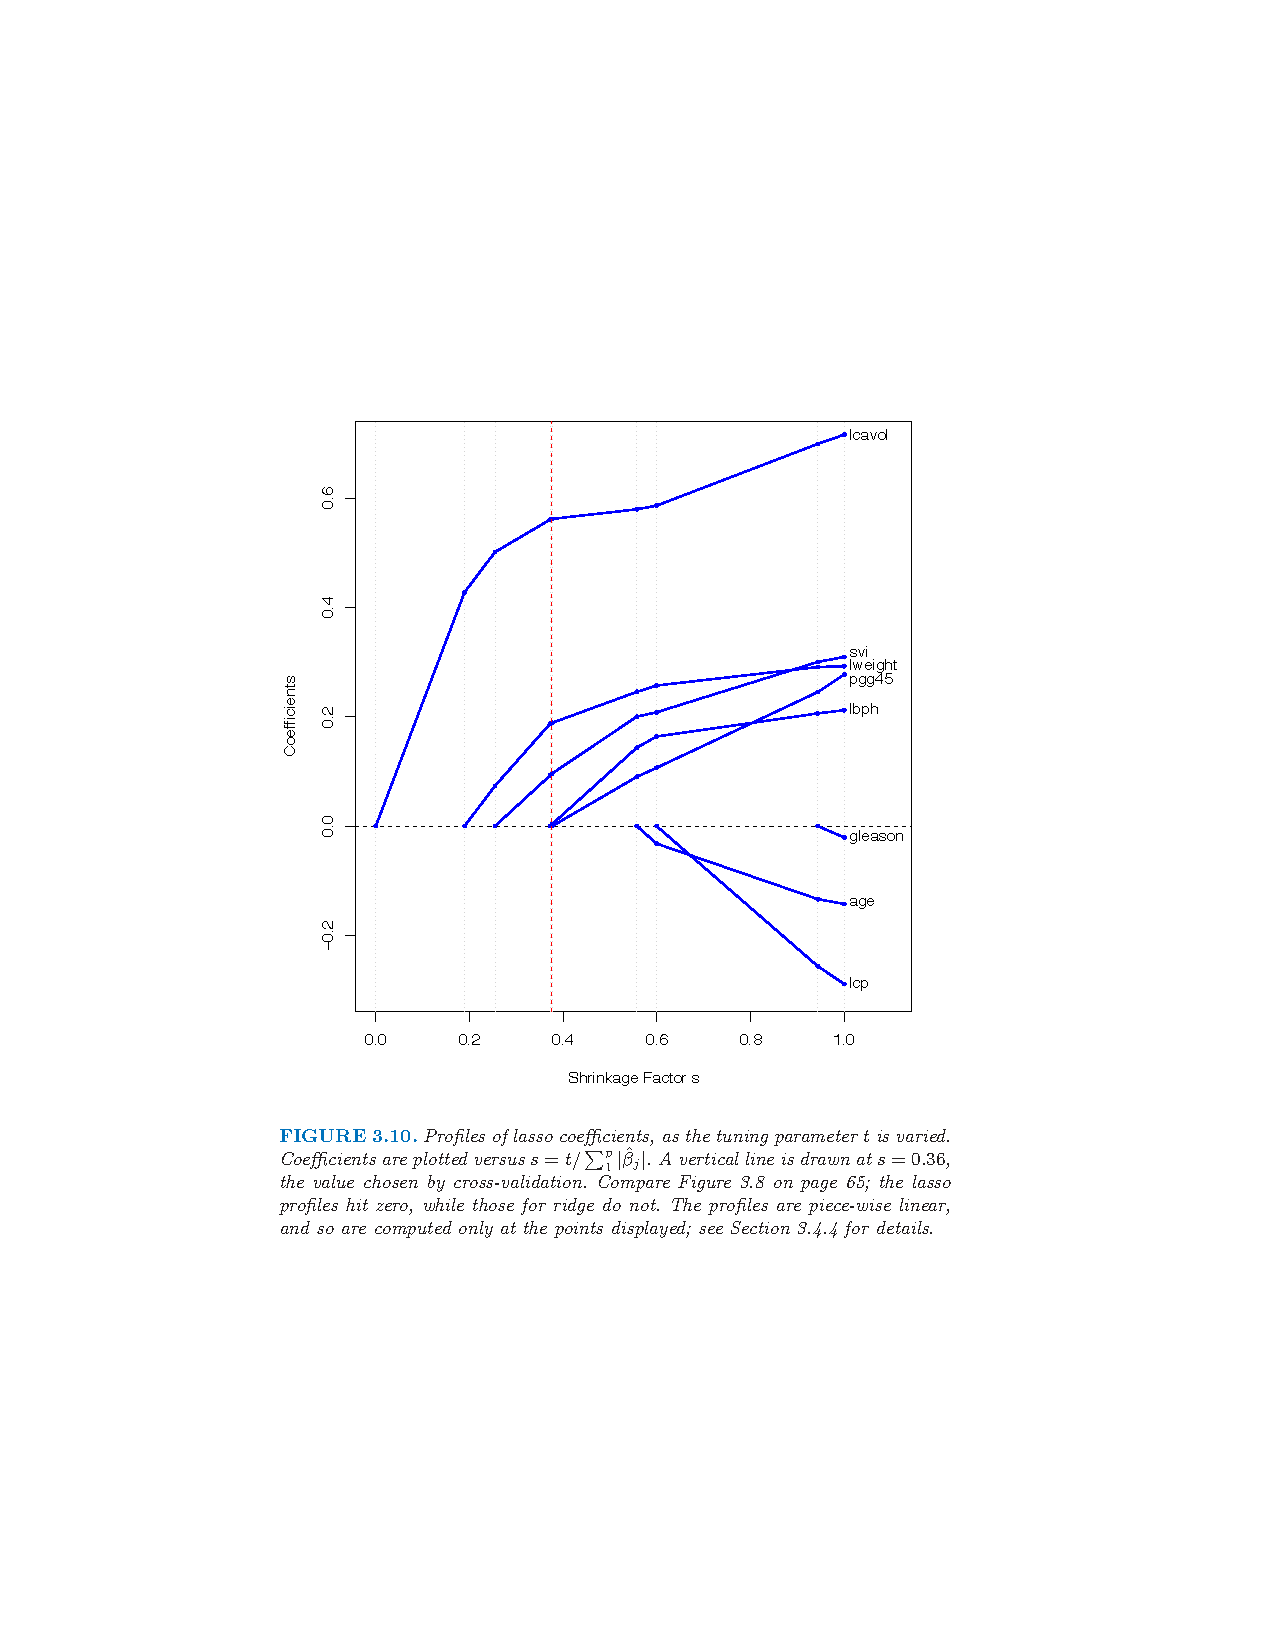
\includegraphics[height=0.9\textheight]{./resources/lassopath}
\end{center}
\end{frame}

\begin{frame}
\frametitle{Ridge Regression}
Another popular alternative is the $q=2$ case
\begin{eqnarray*}
\hat{\beta}^{Ridge} = \arg \min_{\beta} \left[\frac{1}{2} \sum_{i=1}^N (y_i - \beta_0 - \sum_{j=1}^K x_{ij} \beta_j)^2 + \lambda \sum_{j=1}^K | \beta_j|^2 \right]
\end{eqnarray*}
\begin{itemize}
\item Penalty is $L_2$ norm on $\beta$.
\item Can re-write as a constriant  $\sum_{j=1}^K | \beta_j|^2 \leq s$
\item $\hat{\beta}^{Ridge} = (X'X + \lambda I )^{-1} X' Y$.
\item If $X$ is orthonormal then $\hat{\beta}_{j}^{Ridge} =  \hat{\beta}_j /(1 +\lambda )$
\item In words: everything gets dampened by a constant factor $\lambda$ (we don't get zeros).
\item Adding a constant to the diagonal of $(X'X)$ ensures that the matrix will be invertible even when we have multicollinearity.
\end{itemize}
\end{frame}

\begin{frame}
\frametitle{Ridge Path}
\begin{center}
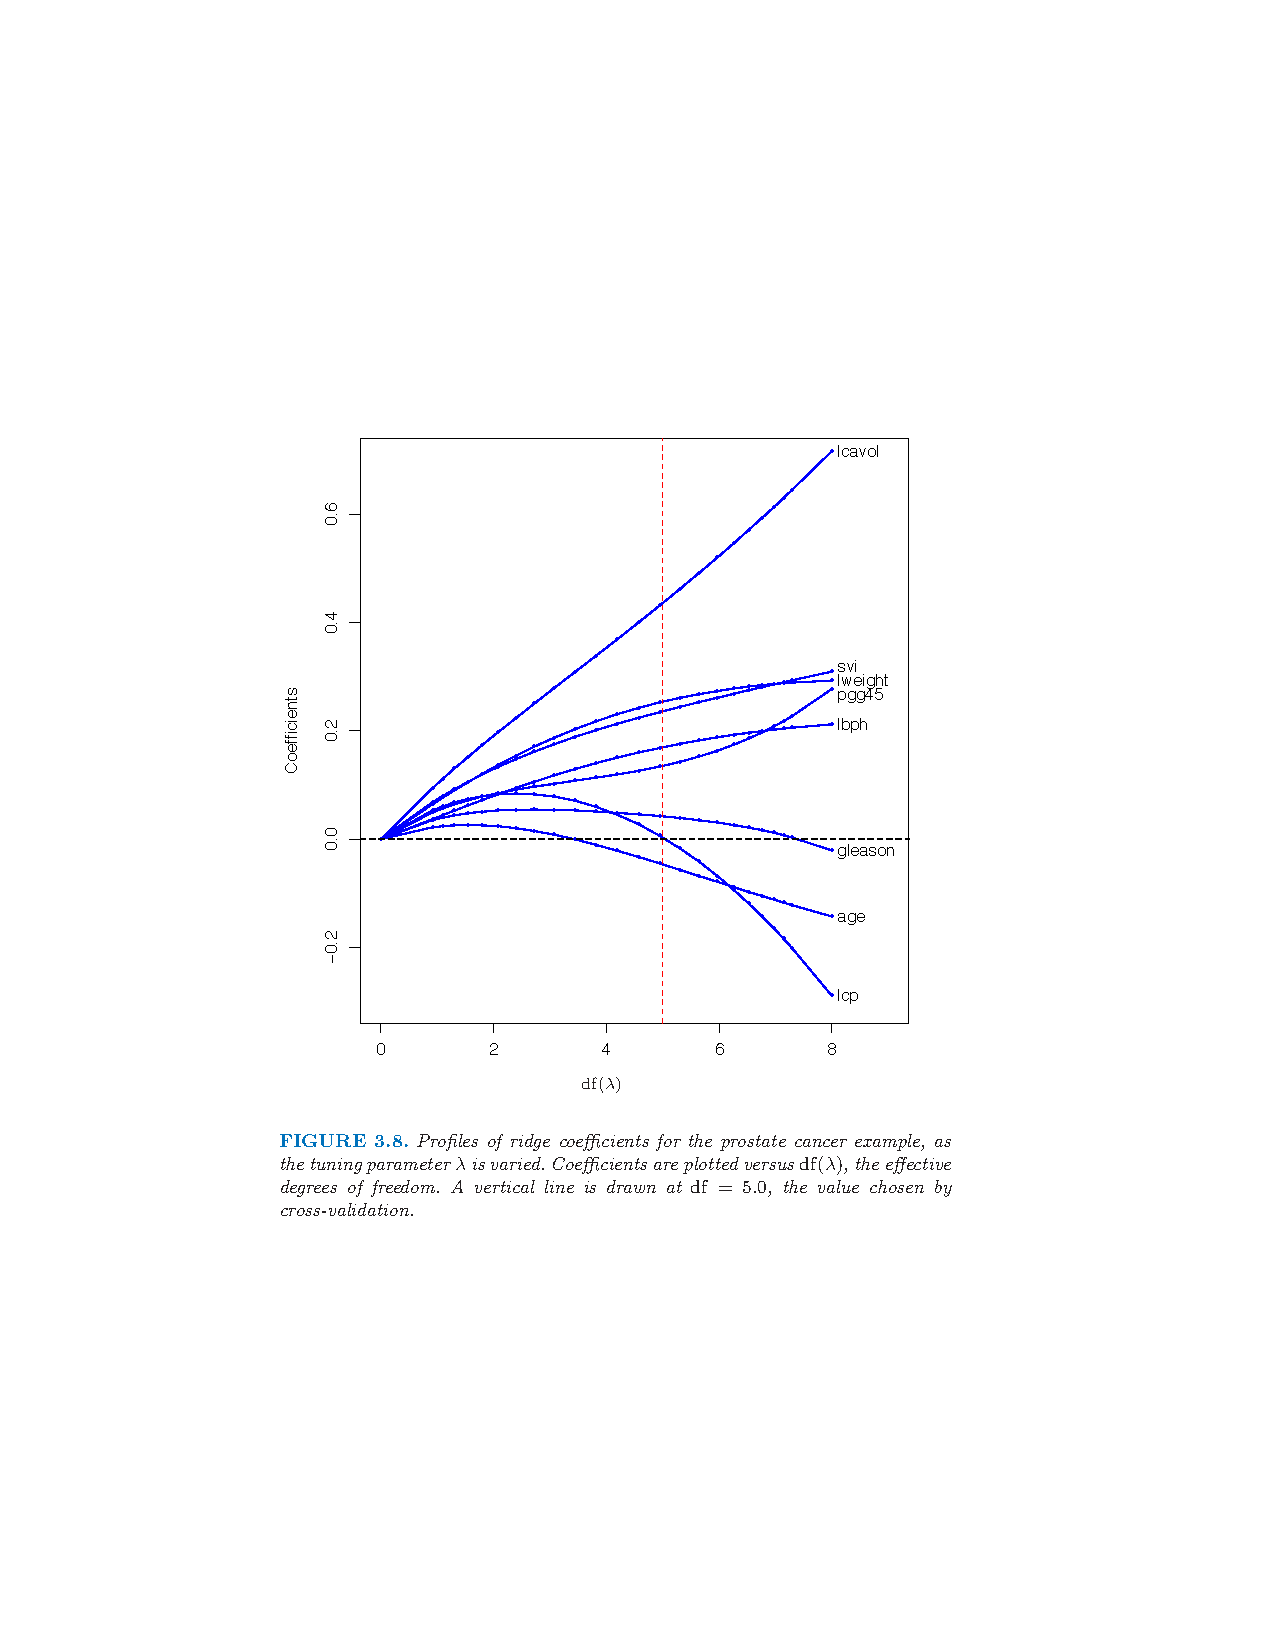
\includegraphics[width=0.85\textheight]{./resources/ridgepath}
\end{center}
\end{frame}

\begin{frame}
\frametitle{LASSO vs Ridge}
\begin{center}
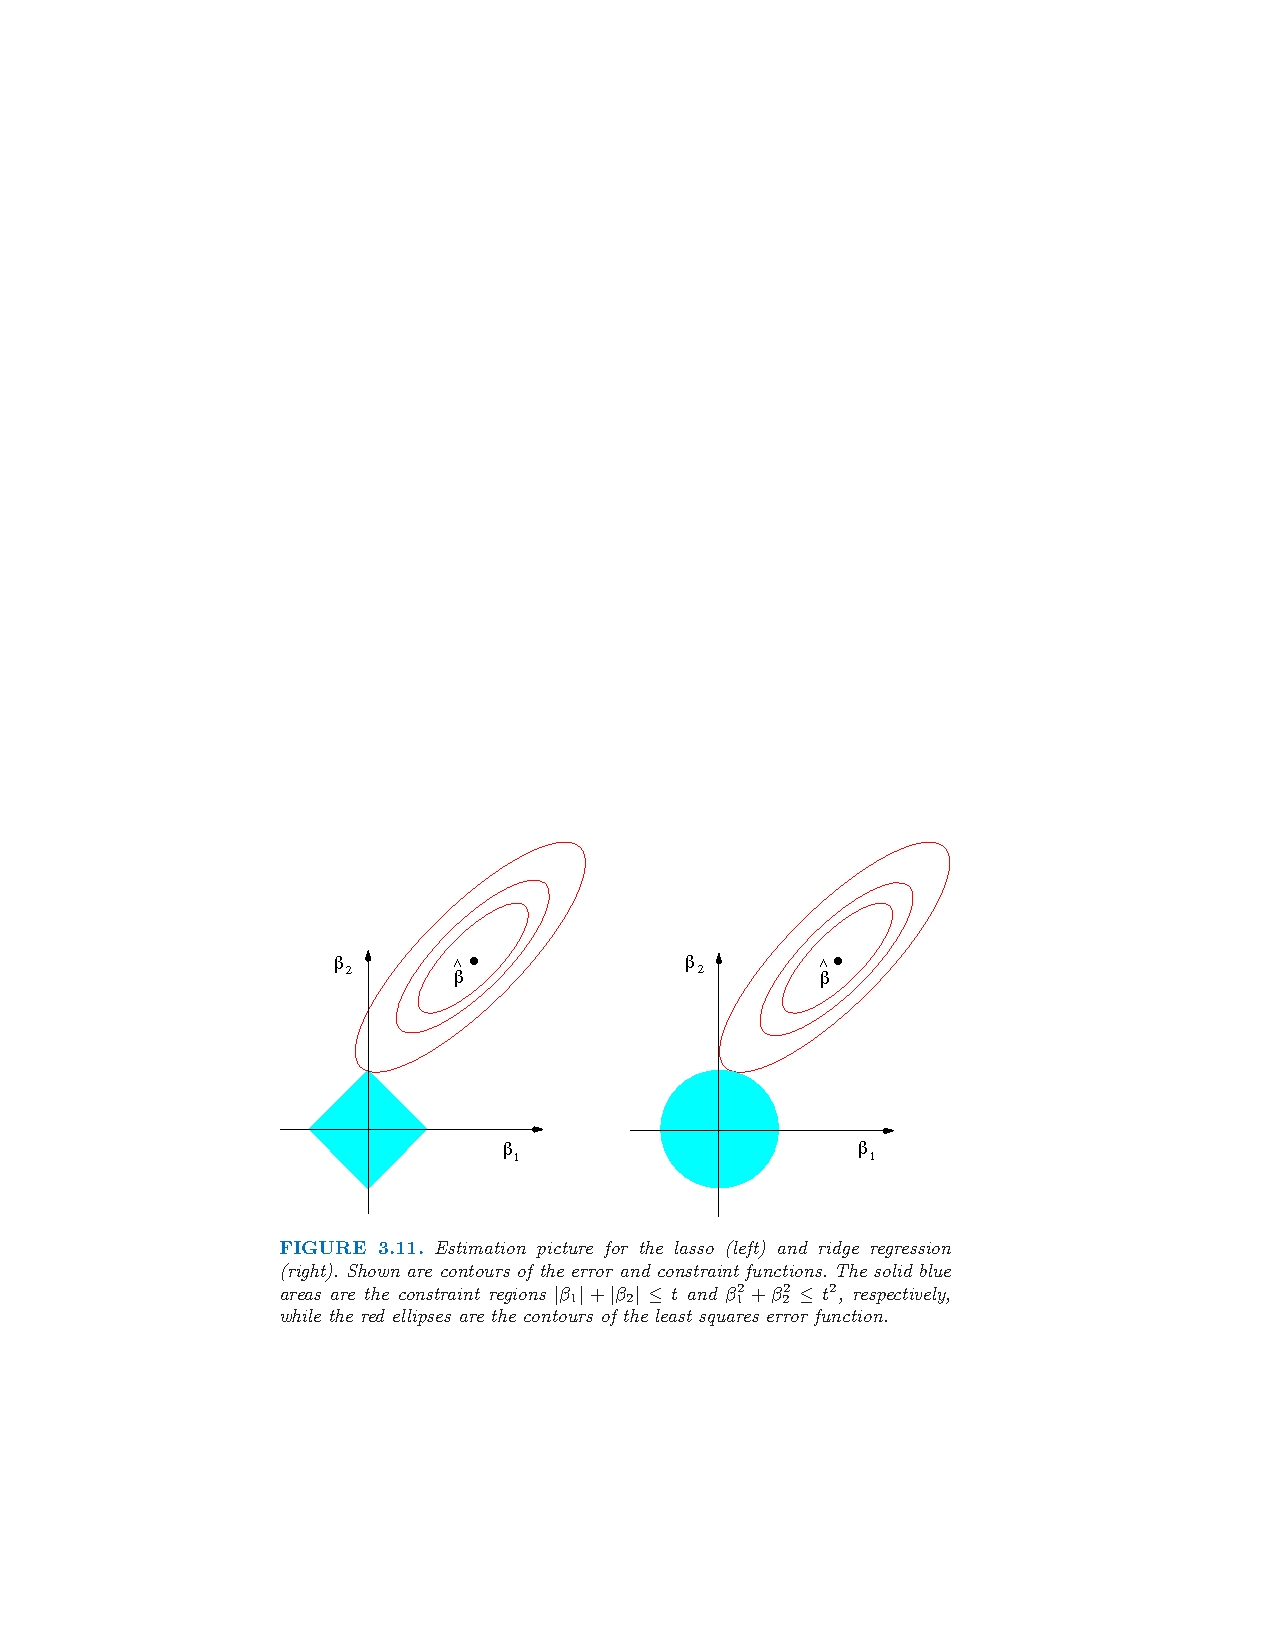
\includegraphics[width=\textheight]{./resources/geometry}
\end{center}
\end{frame}

\begin{frame}
\frametitle{What is the point?}
\footnotesize
Ridge:
\begin{itemize}
\item Ridge doesn't provide sparsity which can be a good thing.
\item It is most helpful (relative to OLS) when $X$'s are highly correlated with one another.
\item OLS can set large but imprecise coefficients when it cannot disentangle effects.
\end{itemize}
LASSO:
\begin{itemize}
\item LASSO is useful for variable/feature selection.
\item LASSO does not generally posses the \alert{oracle property} though variants such as \alert{adaptive LASSO} may.
\item LASSO sometimes has the oracle property for $p \gg N$ and cases where the true $\beta$'s are not too large.
\item People sometimes use LASSO to choose components and then OLS for unbiased coefficient estimates
\end{itemize}
\end{frame}

\begin{frame}{Elastic Net}
We can actually combine them using \alert{elastic net regression}:
\begin{eqnarray*}
 P(\lambda_1,\lambda_2,\mathbf{\beta}) =  \lambda _1\sum_{j=1}^K | \beta_j|  +\lambda_2 \sum_{j=1}^K | \beta_j|^2 
 \end{eqnarray*}
 This includes both the $L_1$ and $L_2$ penalties.
\end{frame}

\begin{frame}
\frametitle{LASSO vs. Ridge}
\begin{center}
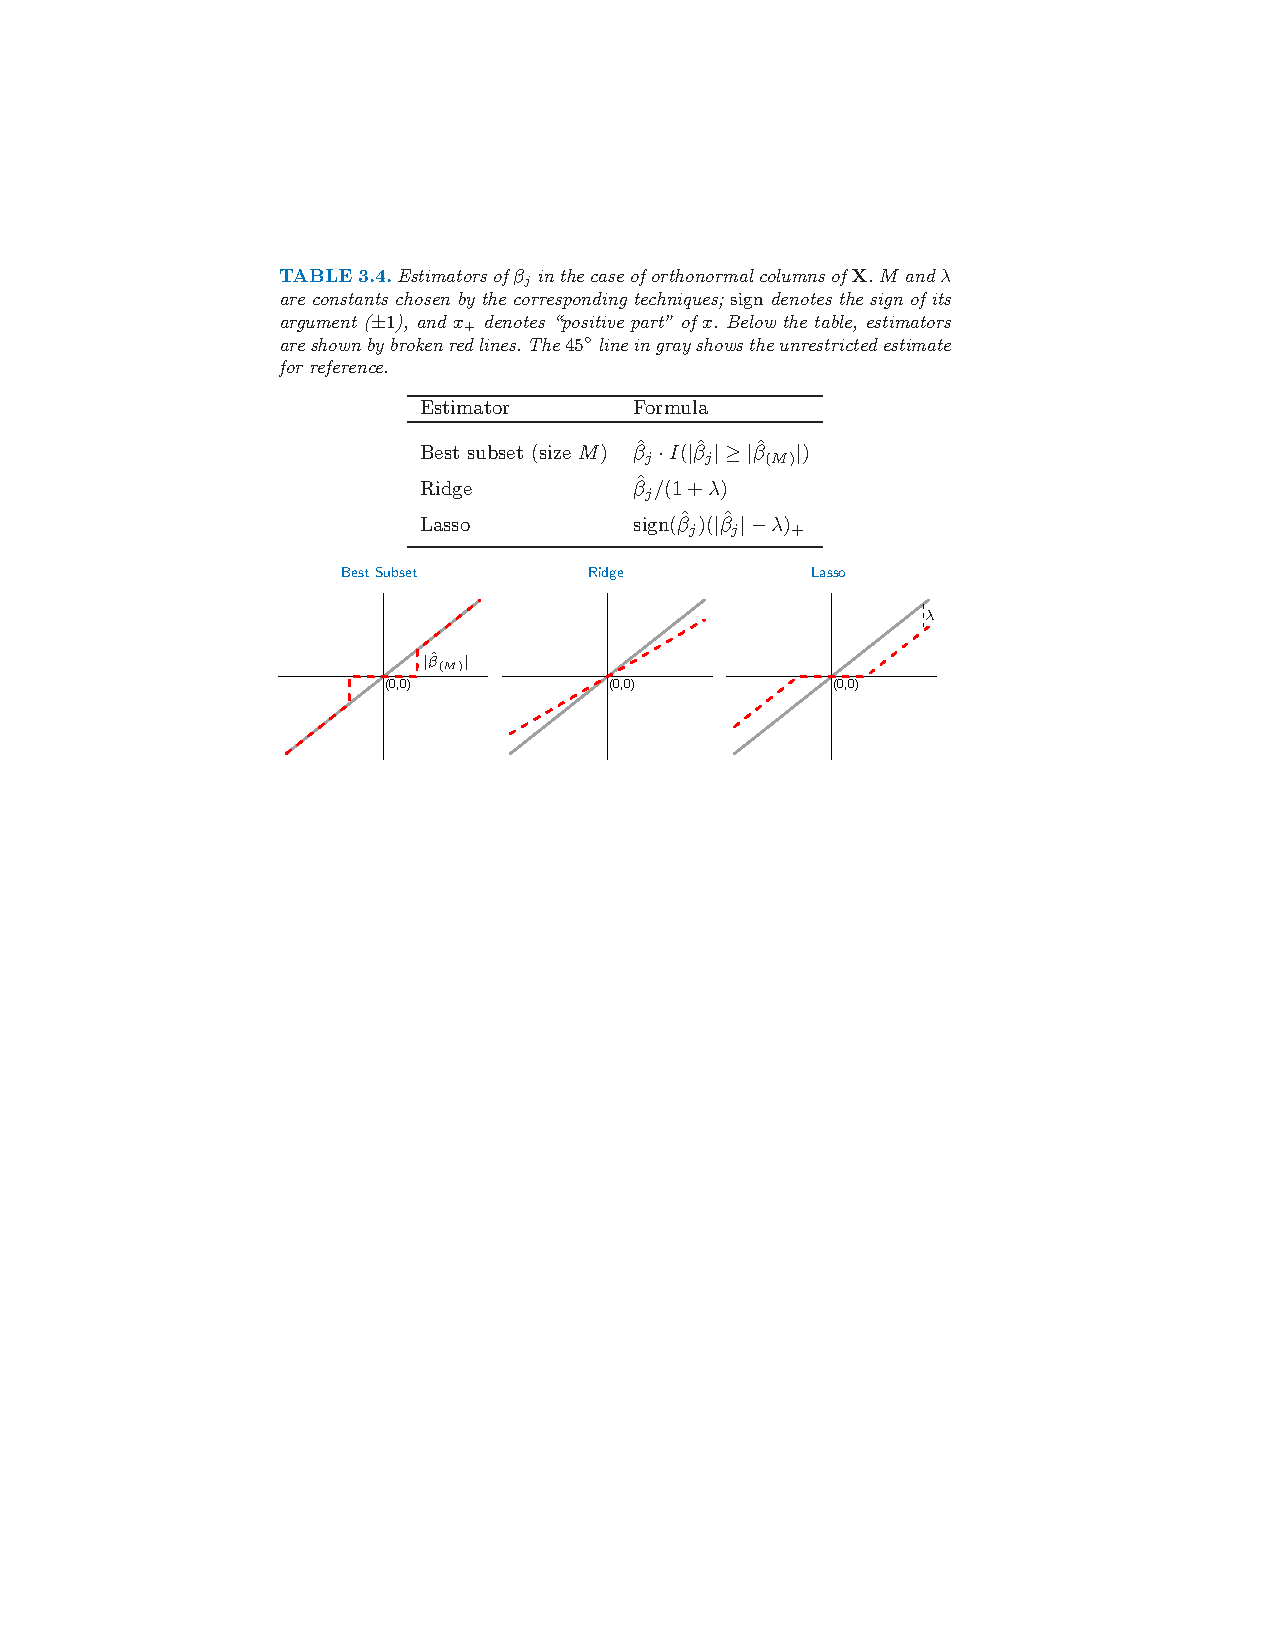
\includegraphics[width=3.5in]{./resources/orthcompare}
\end{center}
\end{frame}


\begin{frame}
\frametitle{LAR: Least Angle Regression}
Remember Forward Stagewise Regression, consider this alternative:
\begin{enumerate}
\item Start with $r= y-\overline{y}$ and $(\beta_1, \ldots, \beta_p) = 0$. (Standardize first!)
\item Find the predictor $x_j$ most correlated with $r$.
\item Move $\beta_j$ from 0 to its least-squares estimate $\langle<x_j , r \rangle$ slowly
\item Update $r \leftarrow r - \delta_j \cdot x_j$.
\item Keep moving $x_j$ in same direction until $x_k$ has as much correlation with updated $r$,
\item Continue updating $(\beta_j, \beta_k)$ in direction of \alert{joint} least-squares coefficients until some other competitor $x_l$ has as much correlation with $r$.
\item Continue until all $p$ predictors have entered. After $\min[N-1,p]$ steps we arrive at full OLS solution.
\end{enumerate}
\begin{itemize}
\item \alert{Optional:} If a current least-squares estimate hits zero drop it from the active set and re-estimate the joint least squares direction without it.
\end{itemize}
\end{frame}


\begin{frame}
\frametitle{LAR: Least Angle Regression}
Why do we need LAR?
\begin{itemize}
\item It turns out that with the optional step from the previous slide: LAR gives us an easy algorithm to compute the LASSO estimate.
\item Actually it does even better -- it gives us the full path of LASSO estimates for all values of $\lambda$!
\item This is actually a relatively new result.
\end{itemize}
\end{frame}


\begin{frame}
\frametitle{LASSO vs LAR}
\begin{center}
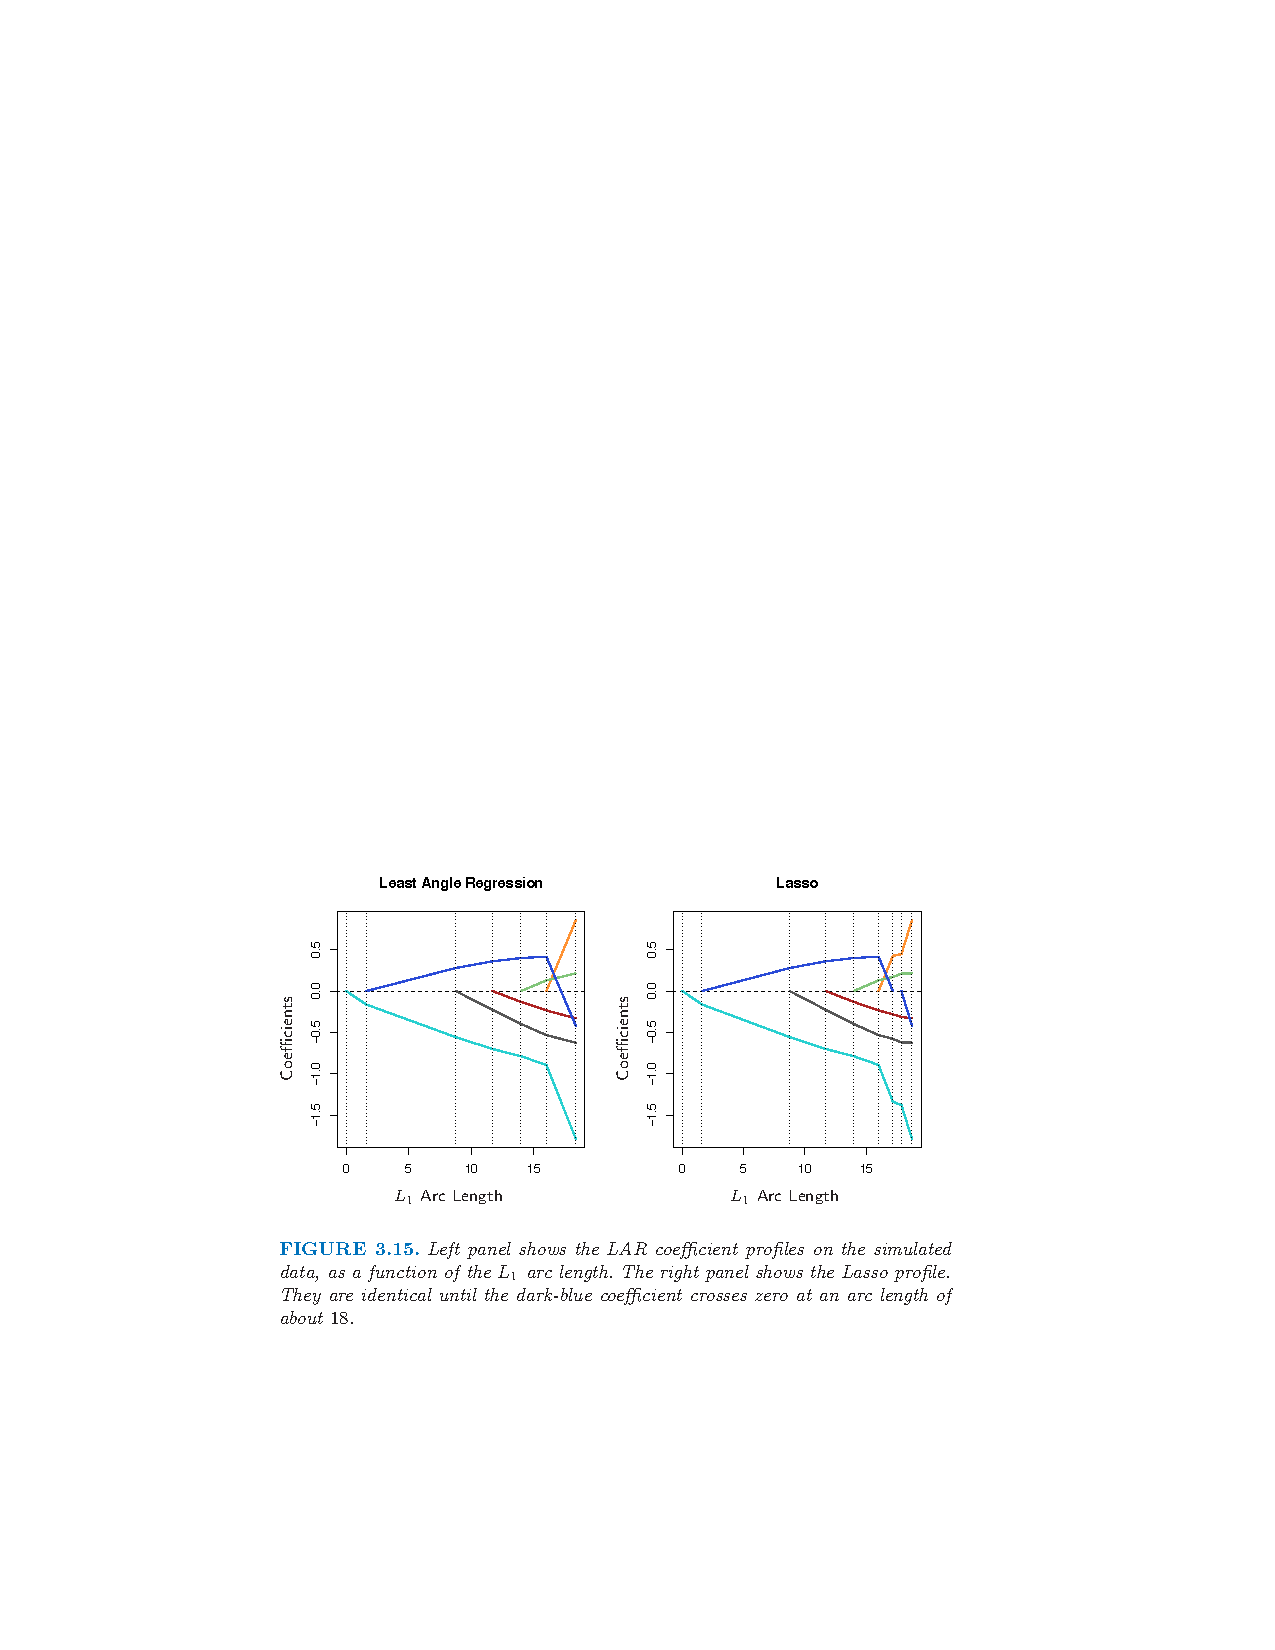
\includegraphics[height=0.9\textheight]{./resources/lar-lasso}
\end{center}
\end{frame}

\begin{frame}
\frametitle{Overall Comparison}
\begin{center}
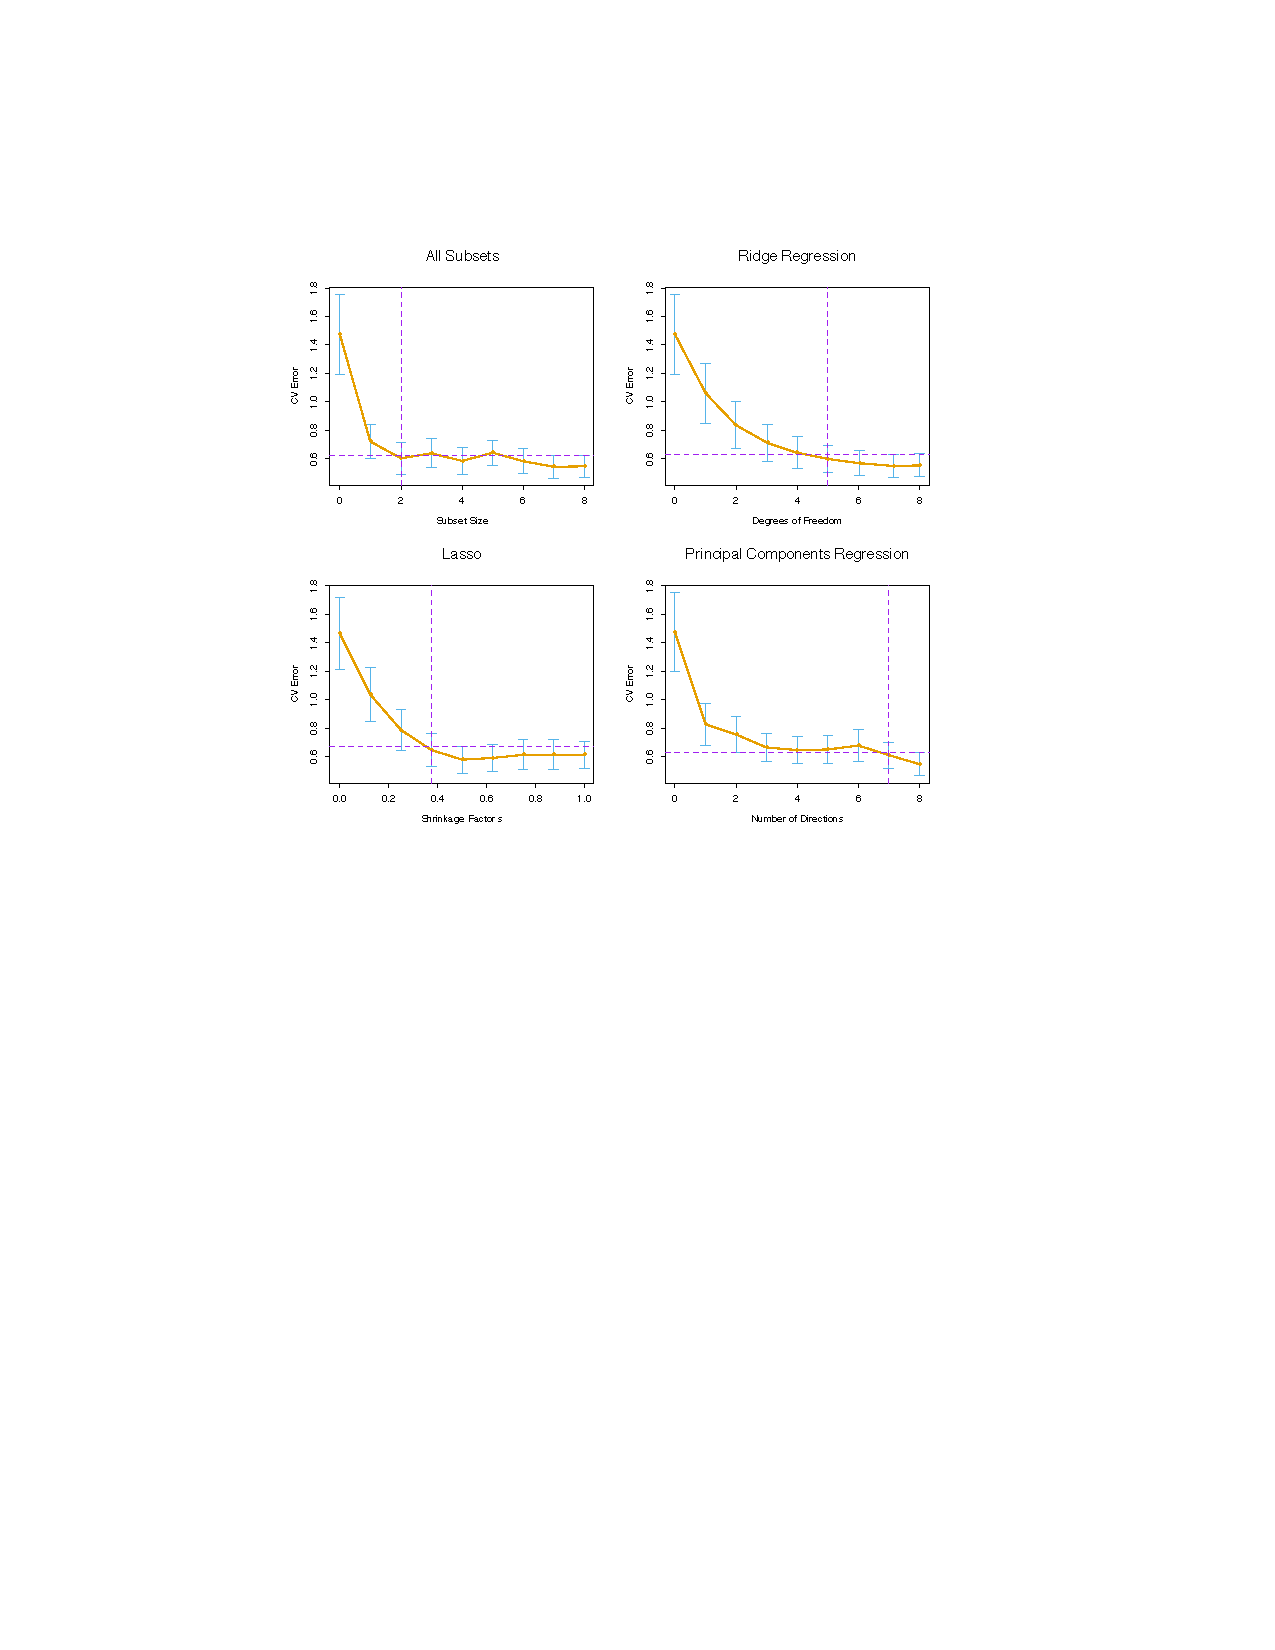
\includegraphics[height=0.9\textheight]{./resources/comparisons}
\end{center}
\end{frame}

\begin{frame}
\frametitle{Overall Comparison}
\begin{center}
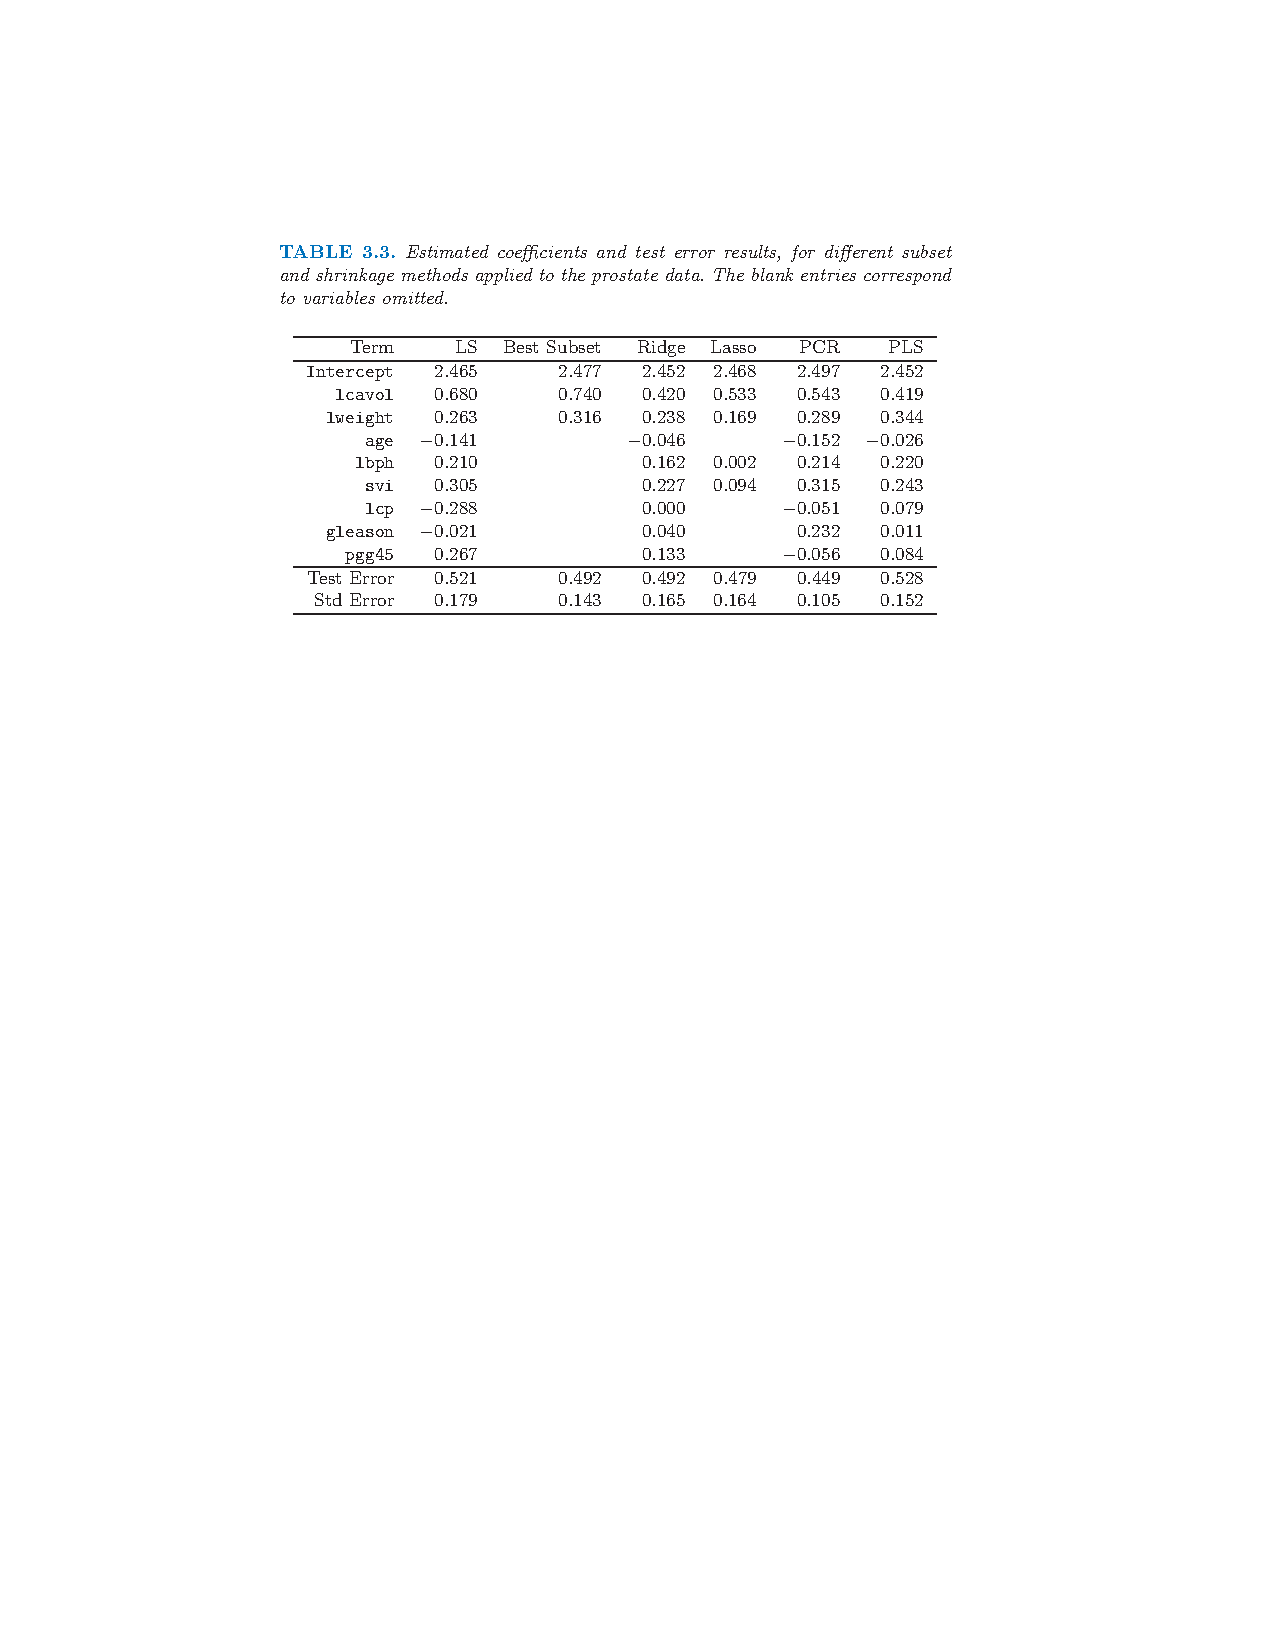
\includegraphics[height=0.9\textheight]{./resources/regressiontable}
\end{center}
\end{frame}


\begin{frame}
\frametitle{Overall Comparison}
\begin{center}
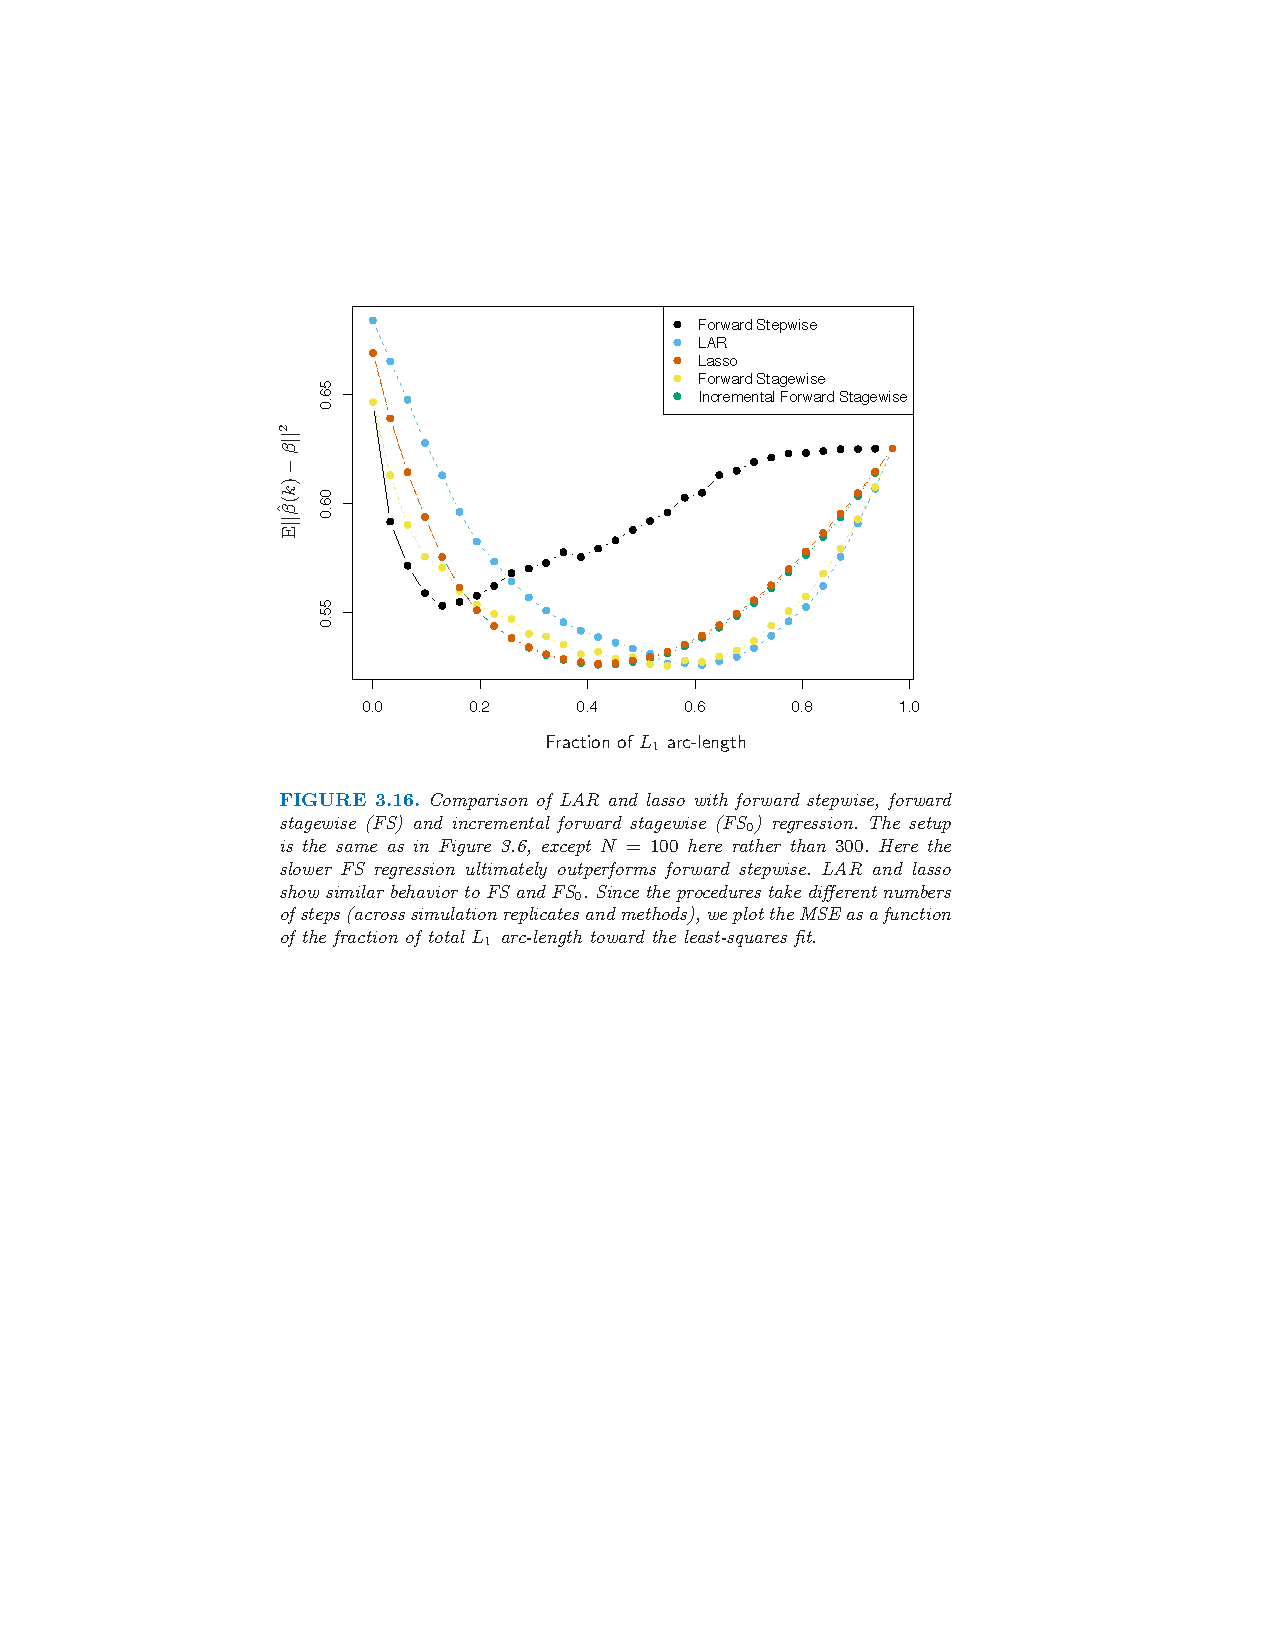
\includegraphics[height=0.9\textheight]{./resources/compareall}
\end{center}
\end{frame}


\begin{frame}
\frametitle{Oracle Property}
\begin{itemize}
\item An important question with LASSO is whether or not it produces consistent parameter estimates (Generally \alert{no}).
\item We think of asymptotics as taking both $N,p\rightarrow \infty$.
\item Donohu (2006) shows that for $p > N$ case, when the true model is sparse, LASSO identified correct predictors with high probability (with certain assumptions on $\mathbf{X}$) as we slowly relax the penalty.
\item Condition looks like (``good'' variables are not too correlated with ``bad'' variables).
\begin{eqnarray*}
\max_{j \in S^{c}} || x_j' X_{S} (X_{S}' X_{S})^{-1} ||_{1} \leq (1 -\epsilon) 
\end{eqnarray*}
\item Where $X_{S}$ are columns corresponding to nonzero coefficients, and $S^{c}$ are set of columns with zero coefficients (at true value).
\end{itemize}
\end{frame}


\begin{frame}
\frametitle{Other Extensions}
\begin{itemize}
\item \textit{Grouped LASSO} for penalzing groups of coefficients at once (like fixed effects)
\item \textit{Relaxed LASSO} run LASSO to select coefficients and then run a non-penalized subset regression or LASSO with a less stringent penalty on the subset. (Here CV tends to pick a less strong penalty term $\lambda$ leading to less shrinkage and bias).
\item \textit{SCAD: Smoothly Clipped Absolute Deviation}: do less shrinkage on big coefficients but preserve sparsity
\begin{eqnarray*}
\frac{ d J_a(|beta,\lambda)}{d \beta} = \lambda \cdot sgn(\beta) \left[ I(| \beta| \leq \lambda) + \frac{(a \lambda - | \beta|)_{+}}{(a-1) \lambda} I (| \beta| > \lambda) \right]
\end{eqnarray*}
\item \textit{Adaptive LASSO} uses  a weighted penalty of the form $\sum_{j=1}^p w_j |\beta_j|$ where $W_j = 1/|\hat{\beta}_j|^{\nu}$ using the OLS estimates as weights. This yields consistent estimates of parameters while retaining the convexity property.
\end{itemize}
\end{frame}

\begin{frame}
\frametitle{Penalty Comparisons}
\begin{center}
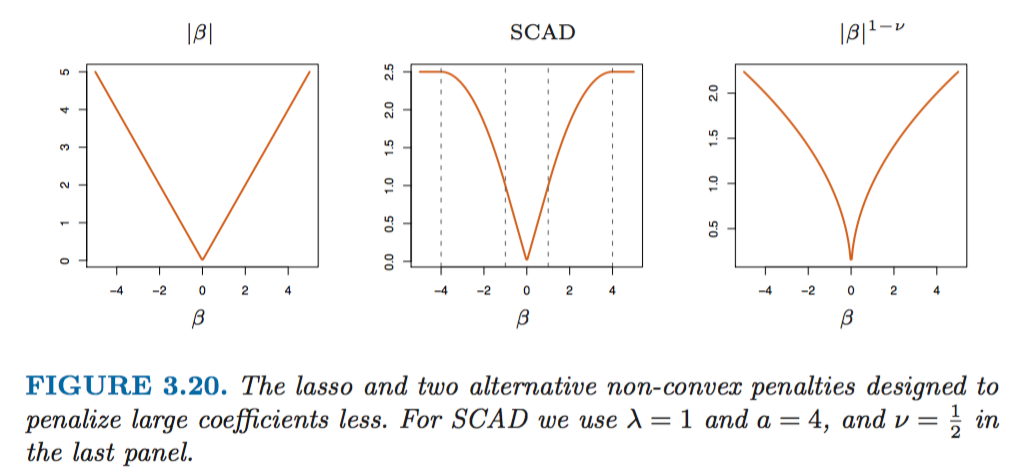
\includegraphics[width=4.5in]{./resources/lassopenalty}
\end{center}
\end{frame}



\begin{frame}
\frametitle{Implementation}
\begin{itemize}
\item Routines are highly specialized: there are lots of tricks
\item No hope of coding this up on your own!
\item In R you can use \texttt{glmnet} or \texttt{lars}.
\item In Python you can use \texttt{scikit-learn}
\item In most recent Matlab in Stats toolbox you have \texttt{lasso} and \texttt{ridge}.
\item In STATA you can download \texttt{.ado} files from Christian Hansen's website (Chicago).
\end{itemize}
\end{frame}



\end{document}
